%%===================Método proposto==============%%
\section{Método Proposto}
\frame{
  \frametitle{Método Proposto}
   

      	\begin{itemize}
      	 \item Esta proposta visa a aplicação da EG para geração de heurísticas
      	 de alto nível para uma plataforma hiper-heurística para o PDP (HyPDP).
      	 \item Baseada no trabalho desenvolvido por Sabar et al. \cite{sabar2015automatic}.
      	 \item No contexto desta proposta:
      	   \begin{itemize}
	      	 \item Heurísticas de alto nível consistem de um \textbf{mecanismo de seleção} e um \textbf{critério de aceitação}. 
	      	 \item Heurísticas de baixo nível são compostas por um conjunto de heurísticas, selecionadas de
	      	 estudos anteriores, um mecanismo de memória e uma função para avaliar as soluções ao PDP.
      	   \end{itemize}
      	\end{itemize}

}

\frame{
	\frametitle{Método Proposto}

		\begin{figure}[!htb]
			\centering
			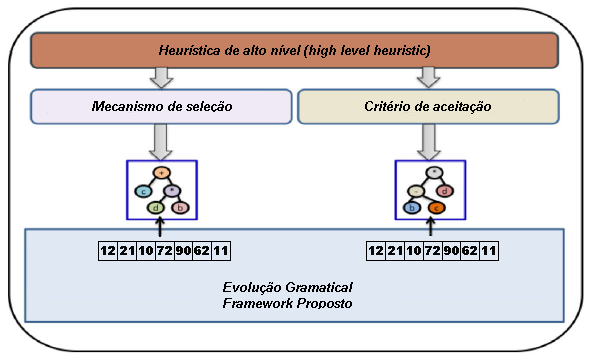
\includegraphics[scale=.8]{figuras/ProposedFramework.png}
			\caption{Método proposto}
			\label{fig:proposedFramework}
		\end{figure}	

}



\begin{frame}{Terminais para gerar mecanismos de seleção}
	

		\begin{itemize}
			\item RC (\textit{Reward Credit}): Recompensa que uma determinada heurística de baixo nível deve receber baseado no seu desempenho.
			% O cálculo da melhoria é dado por: $M(i) = (|f1 -f2|/f1) *100$ se $f2 < f1$, onde $f1$ é a qualidade da solução corrente e $f2$ é a qualidade da solução resultante. 
			%A melhoria obtida é salva em uma janela deslizante (FIFO) de tamanho W. O crédito de qualquer heurística de baixo nível é então atribuído como o máximo valor na janela deslizante correspondente. 
			%A ideia por trás deste critério é: heurísticas de baixo nível que não são usadas com frequência mas que alteram a solução com grandes melhorias tendem a ter mais preferência do que aquelas que geram pequenas melhorias. Portanto as heurísticas que trazem frequentes, mas pequenas melhorias irão ter menos probabilidade de serem selecionadas.
			\item \textbf{$C_{best}$}: Número de vezes que a i-ésima heurística de baixo nível atualizou a melhor solução conhecida. %Este critério favorece as heurísticas de baixo nível que obtiveram êxito em melhorar a melhor solução conhecida até o momento. Este critério é útil para sistematicamente melhorar o atual mínimo local.
			\item $C_{current}$: Número de vezes que a i-ésima heurística de baixo nível atualizou a solução atual. % Este critério favorece as heurísticas de baixo nível que obtém êxito em atualizar a solução corrente. Este critério serve para deixar a busca concentrada próxima à solução corrente.
			\item $C_{accept}$: Número de vezes que a solução gerada pela i-ésima heurística de baixo nível foi aceita pelo critério de aceitação. % Irá favorecer heurísticas de baixo nível que podem ajudar a escapar de um mínimo local.
			\item $C_{ava}$: A média de melhorias anteriores da i-ésima heurística de baixo nível. %Este critério favorece heurísticas de baixo nível que realizaram grandes melhorias em média.
			\item $C_r$: O número de vezes que a i-ésima heurística de baixo nível foi classificada como primeira.
		  
		\end{itemize} 
\end{frame}	
		

\frame{
	\frametitle{Terminais para gerar critérios de aceitação}

	 \begin{itemize}
		 	\item Delta: A diferença da qualidade entre a solução corrente e a solução descendente.
		 	\item PF: A qualidade da solução anterior.
		 	\item CF: A qualidade da solução atual.
		 	\item CI: Iteração corrente.
		 	\item TI: Número de iterações.
	 \end{itemize}
		
		

}



\frame{
	\frametitle{Funções matemáticas para gerar as heurísticas de alto nível}

		 \begin{itemize}
		 	\item +: Adiciona as duas entradas.
		 	\item -: Subtrai a segunda entrada da primeira.
		 	\item *: Multiplica as duas entradas.
		 	\item \%: Divisão protegida, isto é, se o denominador for 0, o altera para 0,001.
		 \end{itemize}

}


\subsection{Gramática Proposta}
\frame{
	\frametitle{Gramática Proposta}
	
	\begin{figure}[!htb]
		\centering
		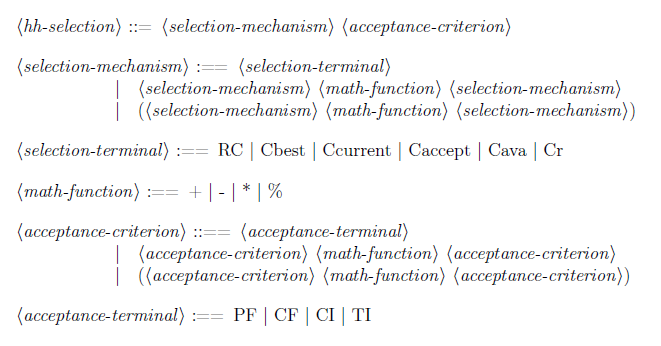
\includegraphics[scale=.6]{figuras/ProposedGramatica.png}
		\caption{Gramática para converter vetores de inteiros em heurísticas de alto nível.}
		\label{fig:proposedGrammar}
	\end{figure}
	
	
}


\subsection{EG para gerar heurísticas de alto nível}
\frame{
	\frametitle{EG para gerar heurísticas de alto nível}
	

		\begin{itemize}
			\item Utilizando a gramática apresentada e vetores de inteiros é possível gerar heurísticas de alto
			nível.
			
			\item Os conjuntos terminais da gramática apresentam estatísticas sobre as heurísticas de
			baixo nível e estas são a matéria-prima para a construção dos componentes das heurísticas
			de alto nível para o HyPDP.
			
			\item O próximo passo consiste em evoluir uma população de vetores de inteiro, gerados de
			maneira aleatória, utilizando o processo evolutivo descrito anteriormente.
		\end{itemize}
		
		

}


\begin{frame}[allowframebreaks]{Função de fitness para a EG}
	\frametitle{Função de \textit{fitness} para a evolução gramatical}
	
			\begin{itemize}
			\item Baseada na função proposta por Sabar et al. \cite{sabar2015automatic}.
			
			\item A probabilidade de selecionar indivíduos é alterada de acordo com a qualidade
			da melhor solução retornada pela execução da plataforma  hiper-heurística HyPDP, utilizando a heurística de alto nível.
			
			\item A
			qualidade retornada pela solução pode ser pior ou melhor do que a solução utilizada como
			entrada para a plataforma hiper-heurística.
		
			\end{itemize}
		

Suponha que $f_i$ e $f_b$ representem a qualidade da solução inicial e da retornada e $Ph[]$ o vetor de probabilidades de seleção dos indivíduos da EG. A retribuição para o $i-$ésimo indivíduo, caso tenha obtido melhoria, será calculada utilizando a equação \ref{eq:fitnessFunction1}.

	\begin{block}{Função de \textit{fitness} para retribuição ao $i-$ésimo indivíduo}
		
		 \begin{equation} {}
		 \label{eq:fitnessFunction1}
		 Ph[i] = Ph[i] + \sigma 
		 \end{equation}
		  Onde:
		 \begin{equation}
					 \sigma = (f_i - f_b)/(f_i + f_b). 
		 \end{equation}		
	\end{block}
	\framebreak
	
	Os demais indivíduos diferentes de $i$ devem receber uma penalização. Suponha que $Nh$ seja o número de indivíduos a penalização é calculada utilizando a equação \ref{eq:fitnessPenalizeFunction1}.
	\begin{block}{Função de \textit{fitness} para penalização aos outros indivíduos $j$}
		\begin{equation} {}
		\label{eq:fitnessPenalizeFunction1}
		Ph[j] = Ph[j] - (\sigma / (Nh - 1))
		\end{equation}
		Tal que:	
		\begin{equation} {}
		\label{eq:fitnessPenalizeFunction2}
		j \in \{1, ..., Nh\} ~e~ j \neq i
		\end{equation}
		
	\end{block}
	
	\framebreak
	
	Caso contrário (se a solução retornada não for melhor que a utilizada como entrada), uma penalização é aplicada ao $i$-ésimo indivíduo utilizando a equação \autoref{eq:fitnessBadFunction1}.
	\begin{block}{Função de \textit{fitness} para penalização do $i-$ésimo indivíduo}
		\begin{equation} {}
		\label{eq:fitnessBadFunction1}
		Ph[i] = Ph[i] - |\sigma \times \alpha|
		\end{equation}
		
		Onde: 
		\begin{center}
			$\alpha =$ iteração corrente $/$ número total de iterações.
		\end{center} 
	\end{block}	

	\framebreak
	
	Os demais indivíduos $j \neq i$ recebem uma recompensa utilizando a \autoref{eq:fitnessOtherFunction} 

	\begin{block}{Função de \textit{fitness} para retribuição dos outros indivíduos $j$}
		\begin{equation} {}
		\label{eq:fitnessOtherFunction}
		 Ph[j] = Ph[j] + (|\sigma| \times \alpha / (Nh -1))
		\end{equation}
		
		 Tal que: 
		\begin{center}
		 $j \in \{1, ..., Nh\} ~e~ j \neq i$
		\end{center} 
		
		Onde:
		\begin{center}
		$Nh$ = número de indivíduos da EG \\ $\alpha =$ iteração corrente $/$ número total de iterações \\
		 $\sigma = (f_i - f_b)/(f_i + f_b)$
			
			
		\end{center}
	\end{block}	
\end{frame}	

\subsection{Conjunto de heurísticas de baixo nível}
\frame{
	\frametitle{Conjunto de heurísticas de baixo nível}		
	\begin{itemize}
		\item \textit{Two Points Crossover} (2X): 
		
		\begin{figure}[!htb]
			\centering
			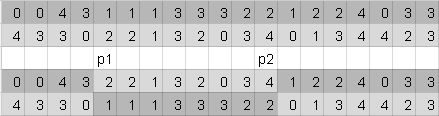
\includegraphics[scale=0.7]{figuras/TwoPointsCrossover.png}
			\caption{Exemplo de aplicação do operador 2x. Fonte Autoria Própria}
			\label{fig:twopointscrossover}
		\end{figure}
		
		
		\item \textit{Multi Points Crossover} (MPX): 
		
		\begin{figure}[!htb]
			\centering
			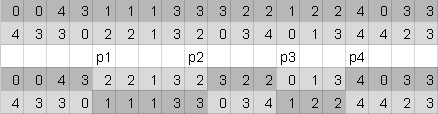
\includegraphics[scale=0.7]{figuras/MultiPointsCrossover.png}
			\caption{Exemplo de aplicação do operador MPX. Fonte Autoria Própria}
			\label{fig:multipointscrossover}
		\end{figure}
		
		
	\end{itemize} 
	
	
}



\frame{
	\frametitle{Conjunto de heurísticas de baixo nível}		
	\begin{itemize}
		
		
	
		\item \textit{Segment Mutation} (SMUT): Altera um número aleatório (5 a 7) de genes consecutivos para direções distintas. 
		
		\begin{figure}[!htb]
			\centering
			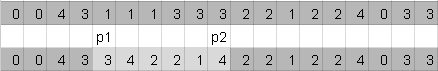
\includegraphics[scale=0.8]{figuras/segmentMutation.png}
			\caption{Exemplo de aplicação do operador SMUT. Fonte Autoria Própria}
			\label{fig:segmentMutation}
		\end{figure}
		
		
		\item \textit {Exhaustive Search Mutation} (EMUT): Esta heurística seleciona um gene aleatório e testa todas as outras direções possíveis e irá manter a alteração que conseguir aumentar a qualidade da conformação.
		
	\end{itemize} 
	
}


\frame{
	\frametitle{Conjunto de heurísticas de baixo nível}		
	\begin{itemize}
		
		
		
	\item \textit{Local Move Operator} (LM): Esta heurística troca direções entre dois genes aleatórios consecutivos.
	
	
	\begin{figure}[!htb]
		\centering
		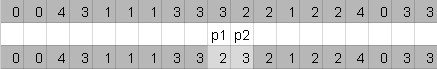
\includegraphics[scale=0.8]{figuras/LocalMoveOperator.png}
		\caption{Exemplo de aplicação do operador LM. Fonte Autoria Própria}
		\label{fig:localMoveOperator}
	\end{figure}
		
		
	\item \textit{Loop Move Operator} (LPM): Esta heurística troca direções entre dois genes que estão a 5 genes de distância na sequência, criando um movimento de \textit{loop}.
	
	
	\begin{figure}[!htb]
		\centering
		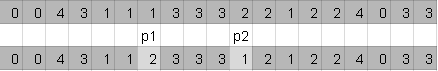
\includegraphics[scale=0.8]{figuras/LoopMoveOperator.png}
		\caption{Exemplo de aplicação do operador LPM. Fonte Autoria Própria}
		\label{fig:loopMoveOperator}
	\end{figure}	
	\end{itemize} 
	
}




\begin{frame}[allowframebreaks]{Processo geral da EG proposta}	
	
	\begin{itemize}
		\item Gerar população inicial de maneira aleatória e calcular o \textit{fitness} dos indivíduos inserindo-os no HyPDP e executando por um determinado número de iterações.
		\item De maneira iterativa selecionar indivíduos pais e aplicar os operadores
		de cruzamento, \textit{prune}, mutação, e \textit{duplicate} para gerar descendentes. Para avaliar os descendentes, os seguintes passos serão executados:
		\begin{itemize}
			\item Decodificar um indivíduo em uma  heurística de alto nível.
			\item Executar o mecanismo de seleção com objetivo de ordenar as heurísticas de baixo nível.
			\item Selecionar de maneira aleatória uma solução do mecanismo de memória. Aplicar a heurística de baixo nível classificada com maior valor e calcular a qualidade da solução gerada.
			\item Se a solução gerada tiver qualidade superior à atual, a atual é substituída. Caso contrário a expressão referente ao critério de aceitação será executada.A  solução gerada pela
			heurística de baixo nível é aceita baseada no valor retornado pelo critério de aceitação.
			\item Continuar aplicando  a mesma heurística de baixo nível repetidamente até que não ocorram mais melhorias.
			\item Se não houverem mais melhorias, troca-se a heurística de baixo nível atual pela
			segunda melhor classificada.
			\item Se a etapa anterior chegar ao fim da lista de heurísticas de baixo nível, é executado o
			mecanismo de seleção novamente e a lista de heurísticas de baixo nível é reordenada.
			A busca reinicia agora utilizando a heurística de baixo nível melhor classificada.
			\item O HyPDP continuará utilizando as heurísticas de alto
			nível por um tempo pré-determinado
			de iterações.
			\item A solução gerada ao final da busca será avaliada para
			entrar ou não no mecanismo de memória.
		\end{itemize}
		\item O processo da EG só irá terminar quando o critério de parada for atingido e será retornado o indivíduo (heurística de alto nível) que possuir o maior \textit{fitness}. Também será retornada a solução do mecanismo de memória que tiver a maior qualidade.
	\end{itemize}

\end{frame}



\begin{frame}[allowframebreaks]{Mecanismo de Memória}	
	
	\begin{itemize}
		\item Baseado no trabalho de Sabar et al. \cite{sabar2015automatic} um mecanismo de memória será desenvolvido para o HyPDP para armazenar soluções de alta qualidade e diversificadas entre si.
		\item A inicialização do mecanismo de memória será feita parte de maneira aleatória e parte utilizando uma estratégia de \textit{backtracking} para garantir que soluções válidas sejam geradas.
		\item A atualização do mecanismo de memória irá ocorrer toda vez que o HyPDP terminar a busca. 
		\item Para uma solução entrar no mecanismo de memória sua qualidade e sua diversidade irão ser avaliadas: a qualidade da solução é dada pela quantidade de iterações H-H multiplicada por -1. \item Para avaliar a diversidade será utilizada a distancia de \textit{Hamming}.
	
		
			
	\end{itemize}
	
\end{frame}



\begin{frame}[allowframebreaks]{Avaliação da Abordagem Proposta}	
	

		
		\begin{table}[!htb]
			\scalefont{0.5}
			\begin{center}		
				\label{tab:sequences}
				{$\begin{array}{c r r l}
					\text{Id} & \text{Tamanho} &  \multicolumn{1}{c}{\text{Valor ótimo}} & \multicolumn{1}{c}{\text{Sequência}} \\ \hline
					s1 &20 &-9 & HPHPPHHPHHPHPHHPPHPH \\
					s2 &24 &-9 & HHPPHPPHPPHPPHPPHPPHPPHH \\
					s3 &25 &-8 & PPHPPHHP^4HHP^4HHP^4HH \\
					s4 &36 &-14 &  P^3HHPPHHP^5H^7PPHHP^4HHPPHPP\\
					s5 &48 &-23 &  PPHPPHHPPHHP^5H^{10}P^6 \\
					&   &    &  HHPPHHPPHPPH^5 \\
					s6 &50 &-21 &  HHPHPHPHPH^4PHP^3HP^3HP^4 \\
					&   &    & HP^3HP^3HPH^4{\{PH\}}^4H\\
					s7 &60 &-36 &  PPH^3PH^8P^3H^{10}PHP^3\\
					&   &    &  H^{12}P^4H^6PHHPHP\\
					s8 &64 &-42 &   H^{12}PHPH{\{PPHH\}}^2PPH{\{PPHH\}}^2\\
					&   &    &  PPH{\{PPHH\}}^2PPHPHPH^{12}\\
					s9  &85   &-53  & H^4P^4H^{12}P^6 H^{12} P^3 H^{12} P^3 \\
					&   &    &    H^{12} P^3  H P^2 H^2    P^2 H^2  P^2 H P H  \\
					s10  &100  &-48  &  P^6HPH^{2}P^5H^{3}PH^5PH^{2} P^4 H^{2} \\
					&   &    &   P^2  H^2 P  H^5  P H^{10} P H^{2} P H^{7}  \\
					&   &    &  P^{11} H^{7} P^2  H P   H^3  P^{6} H P H \\
					s11 &100  &-50  &  P^3H^{2}P^2H^{4}P^2H^{3}PH^{2} PH^{2}PH^{4} \\
					&   &    & P^8 H^6 P^{2} H^{6} P^{9} H P H^{2} P  H^{11} P^2  \\
					&   &    &H^3 P  H^{2} P H P^2  H P H^3 P^6 H^3\\ \hline
					\end{array}$}
			\end{center}
				\caption{Sequências que serão utilizadas para avaliar e comparar os resultados obtidos pela abordagem proposta}
		\end{table}

	
\end{frame}


